\documentclass{standalone}

\usepackage{standalone}
\usepackage{tikz}

\begin{document}
    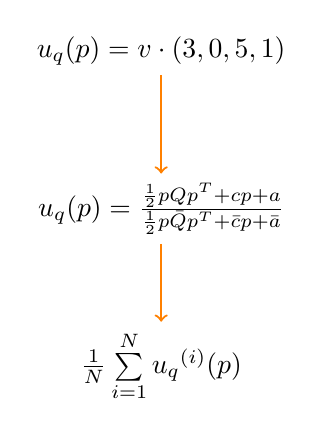
\begin{tikzpicture}
    \node (expr) at (0, 0) {\(u_q(p) = v \cdot (3, 0, 5, 1)\)};

    \pause
    \node (utility) at (0, -2) {\(u_q(p) = \frac{\frac{1}{2}pQp^T + cp + a}
    {\frac{1}{2}p\bar{Q}p^T + \bar{c}p + \bar{a}}\)};
    \draw (expr) edge[->, out=-90, in=90, draw=orange, thick] node[above] {} (utility);
    
    \pause
    \node (tournament) at (0, -4) {\(\frac{1}{N} \sum\limits_{i=1} ^ {N} {u_q}^{(i)} (p)\)};
    \draw (utility) edge[->, out=-90, in=90, draw=orange, thick] node[above] {} (tournament);
    \end{tikzpicture}
\end{document}